\documentclass[spanish]{beamer}
\usepackage{babel}
\usepackage{marvosym} % \MVRIGHTarrow
\usepackage{color, colortbl}
\usepackage{ulem}
% Theme choice:
\usetheme{Madrid}
\usecolortheme{} % beaver, seahorse

% Title page details: 
\title{Desobediencia Tecnológica y Software Libre}

\author{Iván Jijón}
\institute{ FLISoL 2023, Quito - Ecuador}
\date{\today}
\logo{      
    
\includegraphics[width=3.5cm]{img/flisol-banner-social.png}
}

\begin{document}

% Title page frame
\begin{frame}
    \titlepage
\end{frame}


% ToC frame
\begin{frame}{Contenido de la charla}
    \tableofcontents
\end{frame}

% Presentation structure
\section{Definiciones}
    \subsection{Tecnología}
    \subsection{Desobediencia}
\section{¿Qué es \textbf{Desobediencia Tecnológica}?}
    \subsection{Estudio de caso: Cuba durante el Período Especial}
    \subsection{¿Qué \textbf{dificultades} se tuvo que vencer?}
    \subsection{¿Qué actitud ayudó a \textbf{superarlas}?}
\section{En el mundo del Software}
    \subsection{¿Qué dificultades presenta el \textbf{Software Privativo}?}
    \subsection{Breve recordatorio de qué es el \textbf{Software Libre}}
    \subsection{¿Cómo el \textbf{Software Libre} supera esas dificultades?}
\section{Bibliografía y enlaces de interés}
% TODO: Poner los buenos enlaces en cada item del contenido

\begin{frame}{Definiciones}
    \begin{block}{Tecnología - Oxford Languages}
        \begin{enumerate}
            \item Conjunto de los \emph{conocimientos} propios de una técnica.
            \item Conjunto de \emph{instrumentos, recursos técnicos o procedimientos} empleados en un determinado campo o sector.
        \end{enumerate}                             
    \end{block}
    \centering
    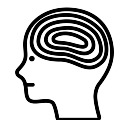
\includegraphics[width=3.5cm]{img/mind.jpg}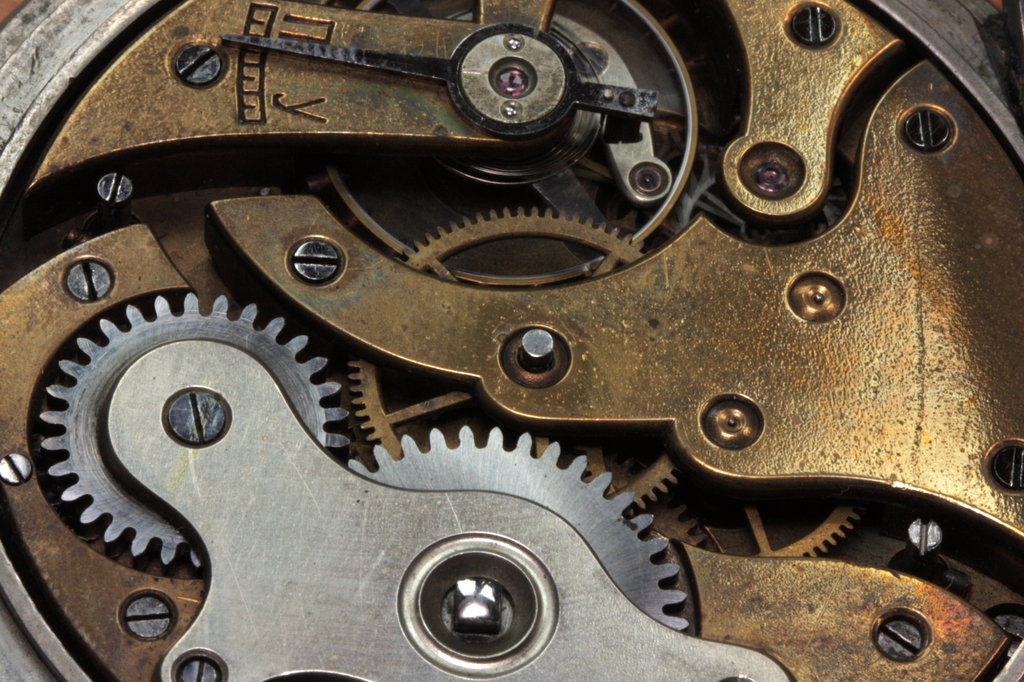
\includegraphics[width=3.5cm]{img/clockwork.jpg}
\end{frame}
\begin{frame}{Definiciones}
    \begin{block}{Desobediencia - Diccionario panhispánico del español jurídico, RAE}
        \begin{enumerate}
            \item Derecho penal: Rechazo activo u omisivo a dar cumplimiento a una orden vinculante y de exigible cumplimiento.
        \end{enumerate}
    \end{block}
    \begin{block}{Artículo 98 - Constitución de la República del Ecuador}
        Los individuos y los colectivos podrán ejercer el derecho a la resistencia frente a acciones u omisiones del poder público o de las personas naturales o jurídicas no estatales que vulneren o puedan vulnerar sus derechos constitucionales, y demandar el reconocimiento de nuevos derechos.
    \end{block}
\end{frame}
\begin{frame}{}
    \begin{quote}
        "La desobediencia es el verdadero fundamento de la libertad. Los obedientes deben ser esclavos." - H.D. Thoreau
    \end{quote}
\end{frame}

\begin{frame}{¿Qué es \textbf{Desobediencia Tecnológica}?}
    El término "Desobediencia Tecnológica" se publica por primera vez por Ernesto Oroza, artista y diseñador cubano en 2009.
    \begin{block}{Desobediencia Tecnológica}
        Un conjunto de acciones creativas producto del cuestionamiento de los objetos y lógicas industriales.    
    \end{block}
    \vspace{0.3cm}
    
    \centering
        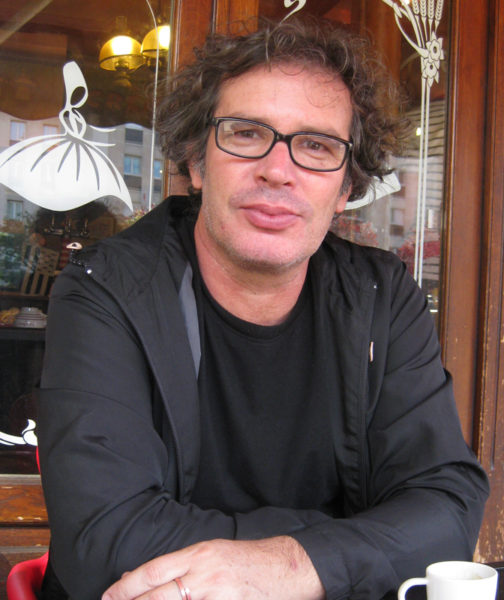
\includegraphics[height=4.5cm]{img/ernestooroza.jpg}
        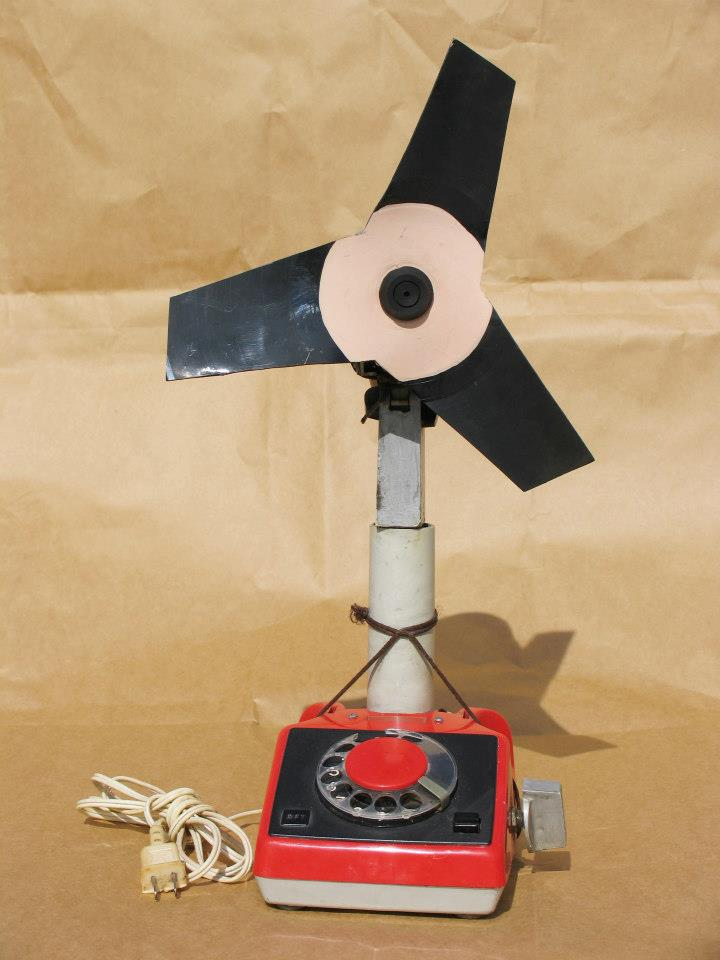
\includegraphics[height=4.5cm]{img/inventos/ventilador.jpg}
        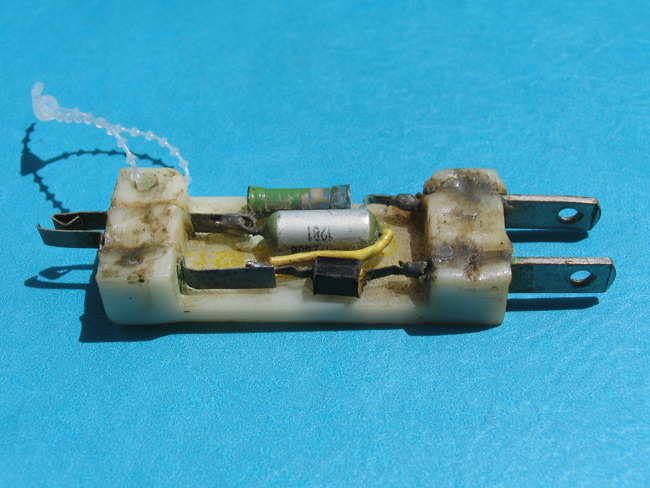
\includegraphics[height=3cm]{img/inventos/battery_charger.jpg}
        
\end{frame}

\begin{frame}{\textbf{Desobediencia Tecnológica}: Contexto}   
    \begin{itemize}        
        \item 1991: caída de la Unión Soviética, economía cubana en implosión.
        \item Se intensifican las necesidades.
        \item El gobierno cubano incita a la gente a trabajar con máquinas: reparar, inventar para responder a la necesidad.        
    \end{itemize}
    \begin{center}            
        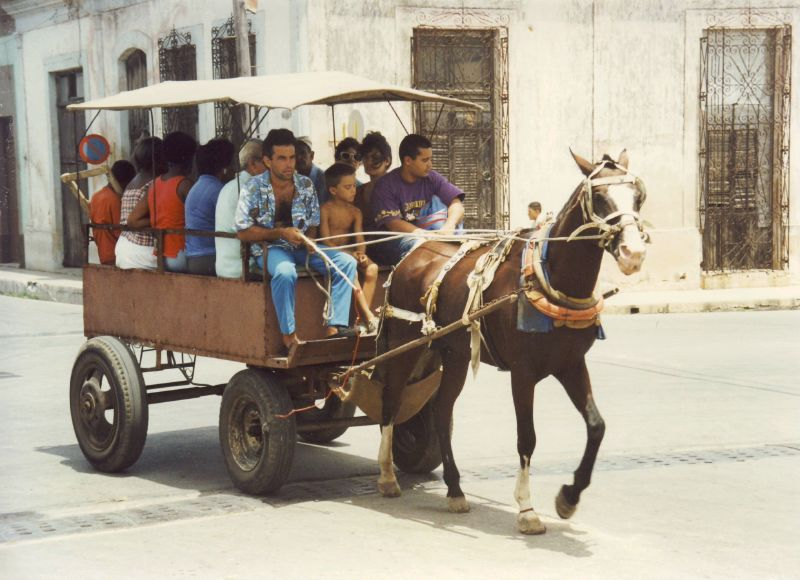
\includegraphics[height=4cm]{img/periodo_especial.jpg}
    \end{center}
\end{frame}

\begin{frame}{\textbf{Desobediencia Tecnológica}: Limitaciones}      
    Dentro de las limitaciones, algunas impuestas por el fabricante, están:
    
    \begin{itemize}
        \item el \textbf{ciclo de vida} de los objetos 
        \item el objeto industrial \textbf{cerrado, hermético}
        \item el diseño no incluye la posibilidad de \textbf{reparar} o de ser \textbf{intervenido} por el usuario
        \item la falta de un \textbf{manual} técnico, además del manual de uso
        \item la \textbf{complejidad} técnica       
    \end{itemize}    
\end{frame}

\begin{frame}{\textbf{Desobediencia Tecnológica}: Comportamiento}        
    El \textbf{ingenio} se posiciona por encima del aparato.
    \vspace{0.3cm}
    \begin{columns}
        \column{0.25\linewidth}
            \centering
            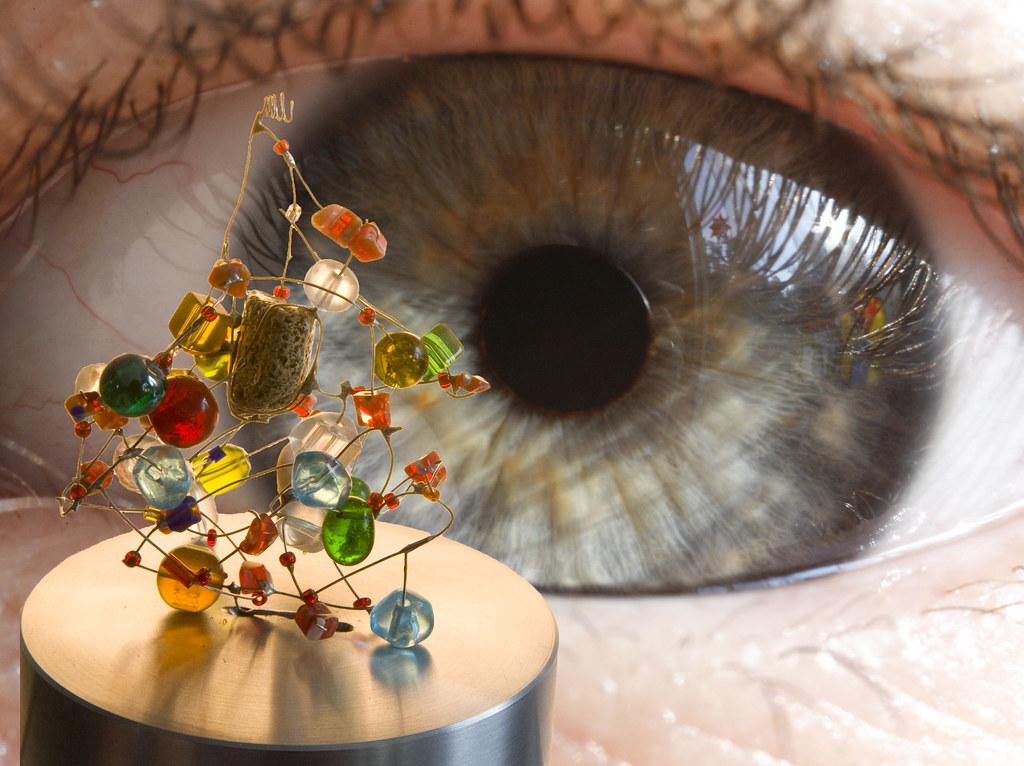
\includegraphics[width=3.5cm]{img/complejidad.jpg}
        \column{0.75\linewidth}
            \begin{itemize}
                \item Nueva mentalidad: ver el objeto por dentro, estudiarlo, entender cada componente.
                \item El aparato deja de ser una entidad única.
                \item Se aprende a reparar, reutilizar, modificar, crear.
            \end{itemize}
    \end{columns}
    \vspace{0.3cm}
    Esto permite saltar las barreras éticas, económicas, legales y estéticas impuestas por los fabricantes.
    Se logra una \uuline{liberación moral}.
\end{frame}

\begin{frame}{\textbf{Desobediencia Tecnológica}: Objetos de la necesidad}
    Ejemplos de objetos de la necesidad:
    \begin{center}            
        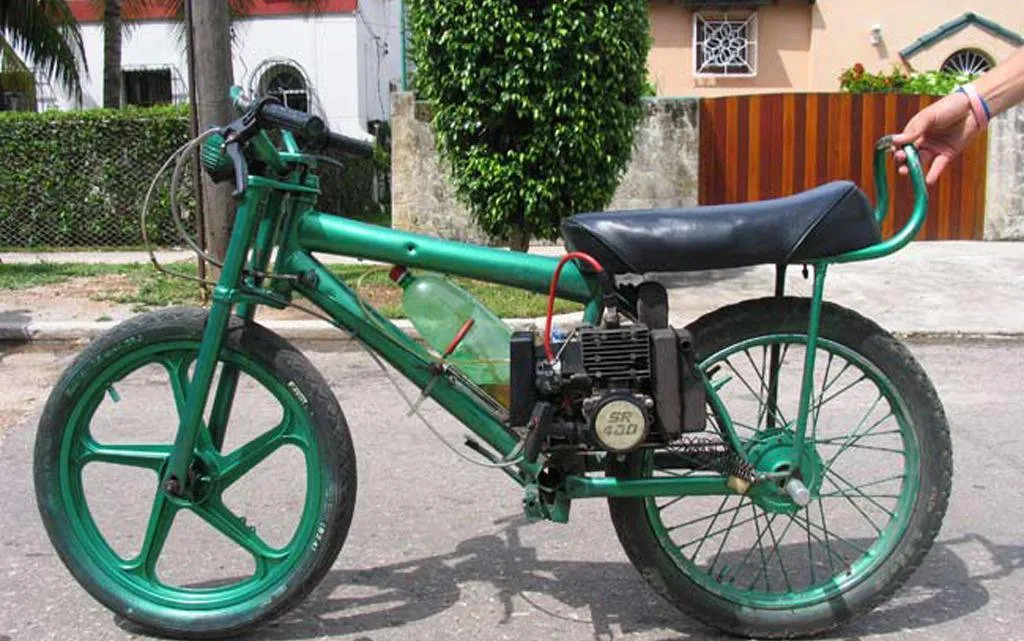
\includegraphics[height=4cm]{img/inventos/rikimbili.jpg}
        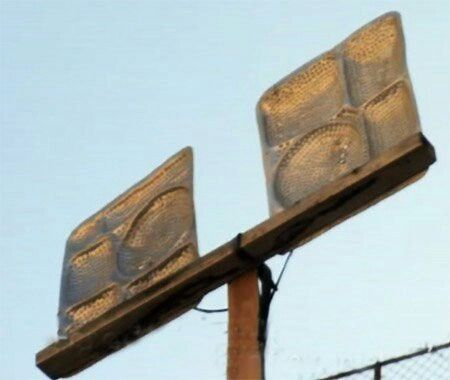
\includegraphics[height=4cm]{img/inventos/antena_bandejas.jpg}
        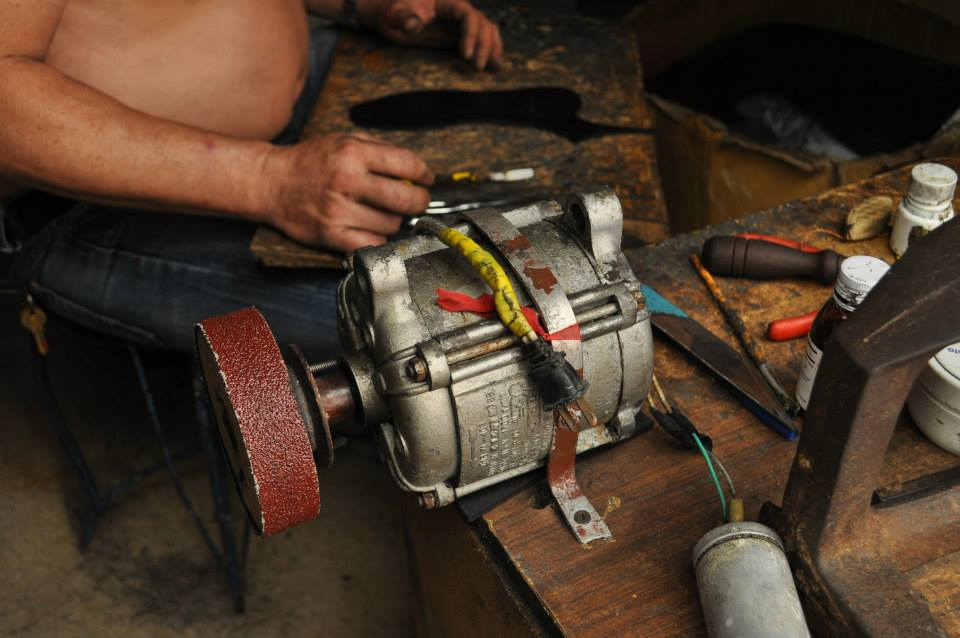
\includegraphics[height=3cm]{img/inventos/motor.jpg}        
    \end{center}
\end{frame}

\begin{frame}
    \begin{quote}
        "La transparencia del objeto otorga características educativas, al decir que un objeto se hace “co-trabajador” señala que este forma parte del oficio, educa, orienta y seguramente estimula también la habilidad creativa, capaz de metamorfosearse, hacer su realidad cotidiana". - Boris Arvatov
    \end{quote}
\end{frame}

\begin{frame}{Dificultades del Software Privativo}
    \centering
    Comparemos el mundo análogo con el mundo del software:
    \vspace{0.6cm}

    \resizebox{11cm}{!}
    {
    \begin{tabular}{|l|l|}
        \hline        
        \rowcolor{lightgray}\textbf{Tecnología Privativa} & \textbf{Software Privativo} \\ 
        \hline
        \hline
        Corto ciclo de vida de los objetos & Viejas versiones obsoletas \\ 
        \hline
        Objeto hermético & El código es inaccesible \\
        \hline
        No se puede reparar / intervenir & El código es inaccesible \\
        \hline
        No hay un manual técnico & No hay documentación técnica \\
        \hline
        Complejidad del aparato & Complejidad del software \\
        \hline
        Funcionalidad limitada & Necesidades no satisfechas \\
        \hline
    \end{tabular}
    }
    
    \vspace{0.6cm}

    ¿Qué respuesta ante estas dificultades? \MVRightArrow{} \textbf{Desobediencia}
    
    ¿Cómo? Gracias al \textbf{Software Libre}.
\end{frame}

\begin{frame}
    \begin{quote}
        "La mayor parte de los hackers tienen en común es la pasión lúdica, la inteligencia y la voluntad de exploración. Podemos decir que el hacking significa explorar los límites de lo posible con un espíritu de sagacidad imaginativa. Cualquier actividad en la que se despliegue esta sagacidad tiene «valor» para el hacker". Richard Stallman
    \end{quote}
\end{frame}

\begin{frame}{Software Libre ("libre" no significa "gratuito")}
    \begin{alertblock}{El Software Libre...}        
        ... no vulnera, rompe, daña, piratea, Software Privativo.        
    \end{alertblock}
    \begin{block}{4 libertades esenciales}
        \begin{itemize}
            \item Libertad 0 - \textbf{Ejecutar} el programa con cualquier propósito.
            \item Libertad 1 - \textbf{Estudiar} cómo funciona el programa, y \textbf{cambiarlo} para que haga lo que se desee.
            \item Libertad 2 - \textbf{Redistribuir} copias para ayudar a otros.
            \item Libertad 3 - \textbf{Distribuir} copias de sus versiones \textbf{modificadas} a terceros.
        \end{itemize}
        
    \end{block}

    \begin{alertblock}{También es un movimiento y una comunidad}        
        No solo es software, es también un \textbf{movimiento} y una \textbf{comunidad}: usuarios, desarrolladores, empresas, diseñadores, pensadores, comunicadores, sociólogos, juristas, profesores, voluntarios, ...
    \end{alertblock}
\end{frame}


\begin{frame}{¿Cómo el Software Libre supera esas dificultades?}
    \centering
    \resizebox{12cm}{!}
    {
    \begin{tabular}{|l|l|}
        \hline        
        \rowcolor{lightgray}\textbf{Software Privativo} & \textbf{Software Libre}\\ 
        \hline
        \hline
        Viejas versiones obsoletas & Mantenimiento: seguridad, funcionalidad \\ 
        \hline
        El código es inaccesible & Es posible estudiar, distribuir \\
        \hline
        No hay documentación técnica & Varios formatos de documentación \\
        \hline
        Complejidad del software & Es posible auditar \MVRightArrow{} mejorar, simplificar, enseñar \\
        \hline
        Necesidades no satisfechas & Es posible adaptar, complementar \\
        \hline
    \end{tabular}
    }
    
    \vspace{0.3cm}
    El usuario es dueño del software (no al revés). 
    
    El software es respetuoso de las libertades del usuario.

    No responde a lógicas autoritarias y códigos cerrados.

    
\includegraphics[width=2cm]{img/GNU_and_Tux.jpg}
    
\includegraphics[width=2cm]{img/latex.jpg}
    
\includegraphics[width=2cm]{img/libreoffice.png}
    
\includegraphics[width=1cm]{img/wahay.jpg}
    
\includegraphics[width=3cm]{img/coyim.jpeg}
    
    
\end{frame}

\begin{frame}{Bibliografía}
    Bibliografía:    
    \begin{itemize}
        \item Desobediencia Tecnológica
        \begin{itemize}            
            \item Cuba's DIY Inventions from 30 Years of Isolation https://www.youtube.com/watch?v=v-XS4aueDUg
            \item https://www.ernestooroza.com/
            \item http://www.technologicaldisobedience.com/
        \end{itemize}
        \item Software Libre  
        \begin{itemize}            
            \item GNU - ¿Qué es el Software Libre? https://www.gnu.org/philosophy/free-sw.es.html
        \end{itemize}      
    \end{itemize}     
\end{frame}

\begin{frame}{Enlaces de interés}
    Enlaces de interés:    
    \begin{itemize}
        \item Cultura Libre  
        \begin{itemize}            
            \item Documental Cultura libre y educación hacker https://vimeo.com/74514091
        \end{itemize}      
        \item Desobediencia Civil
        \begin{itemize}
            \item El derecho a la desobediencia civil en la legislación ecuatoriana:
            https://vlex.ec/vid/derecho-desobediencia-civil-legislacion-876405745
        \end{itemize}
    \end{itemize}    
\end{frame}

\end{document}